\documentclass[11pt,a4paper]{article}
\usepackage{fontspec}
\setmainfont{TeX Gyre Pagella}
\newfontfamily\headfont{Inter}[UprightFont=*-ExtraBold,BoldFont=*-ExtraBold,Extension=.otf,Path=/usr/share/fonts/opentype/inter/]
\usepackage[a4paper,margin=2.3cm]{geometry}
\usepackage{graphicx,booktabs,float,caption,array,xcolor,longtable}
\usepackage[hidelinks]{hyperref}
\usepackage{titlesec}
\usepackage[round]{natbib}
\usepackage{setspace}
\setstretch{1.05}
\renewcommand{\topfraction}{0.9}
\renewcommand{\bottomfraction}{0.8}
\renewcommand{\textfraction}{0.1}
\renewcommand{\floatpagefraction}{0.75}
\setlength{\parindent}{0pt}
\setlength{\parskip}{0.55em}
\titleformat{\section}{\headfont\Large}{\thesection}{0.8em}{}
\titleformat{\subsection}{\headfont\large}{\thesubsection}{0.8em}{}
\captionsetup{font=small,labelfont=bf}
\urlstyle{same}
\hypersetup{pdftitle={Capitals That Moved: Every Capital Move since 1500 in Wikidata, Checked and Corrected},pdfauthor={Tristan Hotham}}

\begin{document}
\begin{center}
{\Large\bfseries Capitals That Moved\par}
\vspace{0.4em}
{\large Every capital move since 1500 in Wikidata, checked and corrected,\\with distances, directions and purpose-built capitals\par}
\vspace{1.2em}
{\large Tristan Hotham\par}
\vspace{0.3em}
{\small Independent researcher\\
ORCID: 0000-0003-4931-9349\\
DOI: \href{https://doi.org/10.5281/zenodo.23847842}{https://doi.org/10.5281/zenodo.23847842}\par}
\vspace{0.8em}
2026
\end{center}

\begin{quote}
\small
\begin{center}\textbf{Abstract}\end{center}
States move their capitals more often than their apparent permanence suggests. I build a table of every move of a state's capital since 1500 that can be read from Wikidata's capital (P36) statements and their start and end qualifiers, and then check, correct and extend it by hand against cited sources. Of 2,978 capital statements for 2,295 states, only 21.3\% carry a start or an end year, and 81\% of present-day sovereign states have a single recorded capital. A transparent set of rules turns dated statements into 202 candidate moves since 1500; after removing 45 wrong or duplicated ones, correcting 5, confirming 22 and adding 42 that Wikidata lacks (Istanbul to Ankara, Kyoto to Tokyo, the wanderings of the Continental Congress and the Province of Canada, among others), the table holds 184 moves by 114 states, 136 lasting and 48 temporary. Every edit is documented with its source. The 20th century has the most moves (59). The median lasting move is 177 km; the longest is the Portuguese court's flight from Lisbon to Rio de Janeiro in 1808 (7,716 km), and the longest lasting move Muscat to Zanzibar in 1840 (3,924 km). 17 moves went to a capital built for the purpose, 12 of them after 1900. Since 1900, 27\% of lasting moves left a coastal capital for the interior, against 8\% before. The status of Indonesia's planned move to Nusantara is reported as of 2026: not made. The results describe the open record as much as history, and I report its gaps throughout.

\textbf{Keywords:} capital cities; capital relocation; planned capitals; historical geography; Wikidata; data quality; open data
\end{quote}

\section{Introduction}
Capital cities look permanent, but many are not old in their role. Brasília was inaugurated in 1960, Abuja replaced Lagos in 1991, Naypyidaw was built in secret and occupied from 2005, and in 2026 Equatorial Guinea moved its capital from Malabo, on the island of Bioko, to Ciudad de la Paz on the mainland. Earlier, Peter the Great built St Petersburg and moved his court there from Moscow, and the Portuguese court ruled an empire from Rio de Janeiro for thirteen years. Capital relocation has a literature of its own, mostly on planned capitals and the motives behind them \citep{rossman,schatz,gordon}, but there is no open, reusable table of every move with its date, distance and direction.

Wikidata \citep{wikidata} comes close. It records the capitals of thousands of states, historical and present, often with the years each held the role. This paper asks how far a complete table of capital moves since 1500 can be read from it, what has to be corrected by hand, and what the resulting table shows: when moves happened, how far they went, which way, and how many went to capitals built for the purpose. An interactive map with a time slider accompanies it (\url{https://maps.tristanhotham.com/moving-capitals/}), and the data, with every manual edit and its source, are released for reuse.

\section{Data}
\subsection{Wikidata}
A query on the QLever Wikidata endpoint \citep{qlever} returned every capital (P36) statement of items that are instances of country, sovereign state, historical country, kingdom, realm, republic, empire, ancient civilisation or constitutional monarchy, with the statement's start time (P580), end time (P582) and rank, the capital's coordinates (P625), the state's inception (P571) and dissolution (P576), and English labels. Collapsed to one record per statement, this gives 2,978 statements for 2,295 states, of which 1,652 existed after 1500. Only 634 statements (21.3\%) have a start or an end year. 4 name an ``unknown value'' capital and 15 are deprecated (including Nusantara for Indonesia and St Petersburg for Russia). Present-day items usually hold only the current capital: of 197 present-day sovereign states, 159 (81\%) have one. Past capitals are more often recorded on items for earlier regimes (the Tsardom of Russia, the Kingdom of Portugal, the British Raj).

\subsection{Other sources}
Natural Earth \citep{naturalearth} provides present-day country borders, land polygons (for distance from the sea) and populated places. The hand checks cite English Wikipedia articles for historical moves and, for 2026, news reports on Equatorial Guinea \citep{africanews} and on Indonesia's Constitutional Court ruling on Nusantara \citep{star,jakpost}. All are listed in the edits file.

\begin{table}[tbp]\centering\small\caption{Hand edits to the automatic table, all listed with reasons and sources in \texttt{data/manual\_edits.csv}.}\label{tab:edits}\begin{tabular}{>{\raggedright\arraybackslash}p{2.4cm}r>{\raggedright\arraybackslash}p{10.2cm}}\toprule Edit & Rows & Examples\\\midrule
Removed & 45 & Wrong order (Herat to Samarkand, 1507); institution not capital (Regensburg, Wetzlar); duplicate with a wrong year (Kraków to Warsaw, 1795); wrong item (West Pakistan); Republic of China and Vichy France statements replaced\\
Corrected & 5 & Moscow to St Petersburg 1730 to 1732; Muscat to Zanzibar 1824 to 1840; Diriyah to Riyadh 1819 to 1824; Helvetic Republic and Central America sequences\\
Confirmed & 22 & Rio to Brasília, Lagos to Abuja, Almaty to Astana, Yangon to Naypyidaw, Melbourne to Canberra and others\\
Added & 42 & Istanbul to Ankara; Kyoto to Tokyo; Karachi to Rawalpindi; Continental Congress 1776 to 1785; Province of Canada 1844 to 1866; Republic of China 1912 to 1949; France 1879 and 1940 to 1944\\
Merged & 1 & The same move on two items with different years, kept once\\
Same place & 14 & Pairs of names for one city (Edo and Tokyo, Constantinople and Istanbul), not counted\\
Relabelled & 29 & Display names only (Fengtian Fu as Mukden, Nan-ching as Nanjing)\\
\bottomrule\end{tabular}\end{table}

\section{Methods}
\subsection{Reading moves from statements}
For each state that existed after 1500, every statement that is not deprecated and names a located capital becomes a spell with a start year and an end year, either of which may be missing. Moves are read in two ways. First, where a spell B starts in year $t$, the old capital A is the other city whose spell ends within two years of $t$ (``both ends dated''); failing that, a city whose spell began before $t$ and has no end (``old capital's end not recorded''); failing that, the city whose spell ended most recently within 30 years before $t$ (``gap''). A city whose spell runs on more than two years past $t$ is treated as a joint capital, not one that was left. Second, where a spell A ends in year $t$ and no move was found at $t$, the new capital is a city with no start date that runs on past $t$, the preferred-rank one if there are several. States whose several capitals have no dates at all (87) cannot be placed in time and are left out.

Moves of under 2 km, and a hand list of pairs that are the same city under two names or two Wikidata items (Edo and Tokyo, Constantinople and Istanbul, Buda and Budapest, Delhi and New Delhi), are set aside as renamings. The same move recorded on several items (both ends within 10 km, years within three) is counted once and the other items are listed with it. This gives 202 candidate moves since 1500 before the hand edits.

\subsection{Checking and correcting by hand}
I checked the moves people know best (Table~\ref{tab:famous}) and every automatic move whose reading looked doubtful against cited sources, mostly English Wikipedia articles, and recorded each decision in \texttt{data/manual\_edits.csv} with a reason and a link (Table~\ref{tab:edits}). Removals fall into four kinds: an undated capital read as the successor when it was the predecessor (Samarkand for the Timurids, Gulbarga for the Bahmanis, Malbork for the Teutonic Order); the seat of an institution read as the capital (the Imperial Diet at Regensburg, the Imperial Chamber Court at Wetzlar); the same move on another item with a different year (Kraków to Warsaw in 1795 rather than 1596; Lisbon to Rio de Janeiro in 1815 rather than 1808); and statements on the wrong item (Pakistan's capitals recorded on the West Pakistan province). Where Wikidata mixes parallel governments (Vichy France and Free France; the Republic of China's overlapping statements for Beijing under several names), I replaced its moves with a checked sequence. Additions cover famous moves Wikidata does not record: Istanbul to Ankara (1923), Karachi to Rawalpindi (1959), Kyoto to Tokyo (1868), the Continental Congress's moves from 1776 to 1785, the Province of Canada's alternating seats from 1844 to 1866, the colonial capitals of Côte d'Ivoire, Belize City to Belmopan (1970), Manila to Quezon City and back (1948, 1976) and Colombo to Kotte (1982). Where I was not sure of a fact, I left Wikidata as it is and let the confidence flag speak.

\subsection{Measures}
Distance is the great-circle (haversine) distance between the two capitals' coordinates on a sphere of radius 6{,}371 km; direction is the initial bearing, binned into eight compass points. Each move is assigned to the present-day country where most of its state's capitals lie (Natural Earth). Distance from the sea is to the nearest point of the Natural Earth 1:50m land outline, so inland seas and lakes such as the Caspian and Lake Tanganyika do not count. For moves within one present-day country I also compute the change in distance to the centroid of the country's largest polygon. A move is temporary if the new seat was held for less than a year, if the capital was back in the starting city within ten years, or if it is a wartime or exile seat in a short hand list (the Portuguese court in Rio, the Sardinian court in Cagliari, Indonesia's revolutionary capitals, Prussia's refuge in Memel). Purpose-built capitals are a hand list of cities founded, or laid out as new towns, to be capitals \citep{wikiplanned}. Each move carries a confidence flag: checked (confirmed or added by hand from a cited source), high (both ends dated consistently in Wikidata), medium (one end dated) or low (a gap).

\section{Results}
\subsection{How many, and when}
The table holds 184 moves since 1500 by 114 states in 66 present-day countries: 136 lasting and 48 temporary (Figure~\ref{fig:map}). 142 come from Wikidata (of them 111 with both ends dated) and 42 were added by hand; 69 in all are checked against a source.

\begin{figure}[tbp]\centering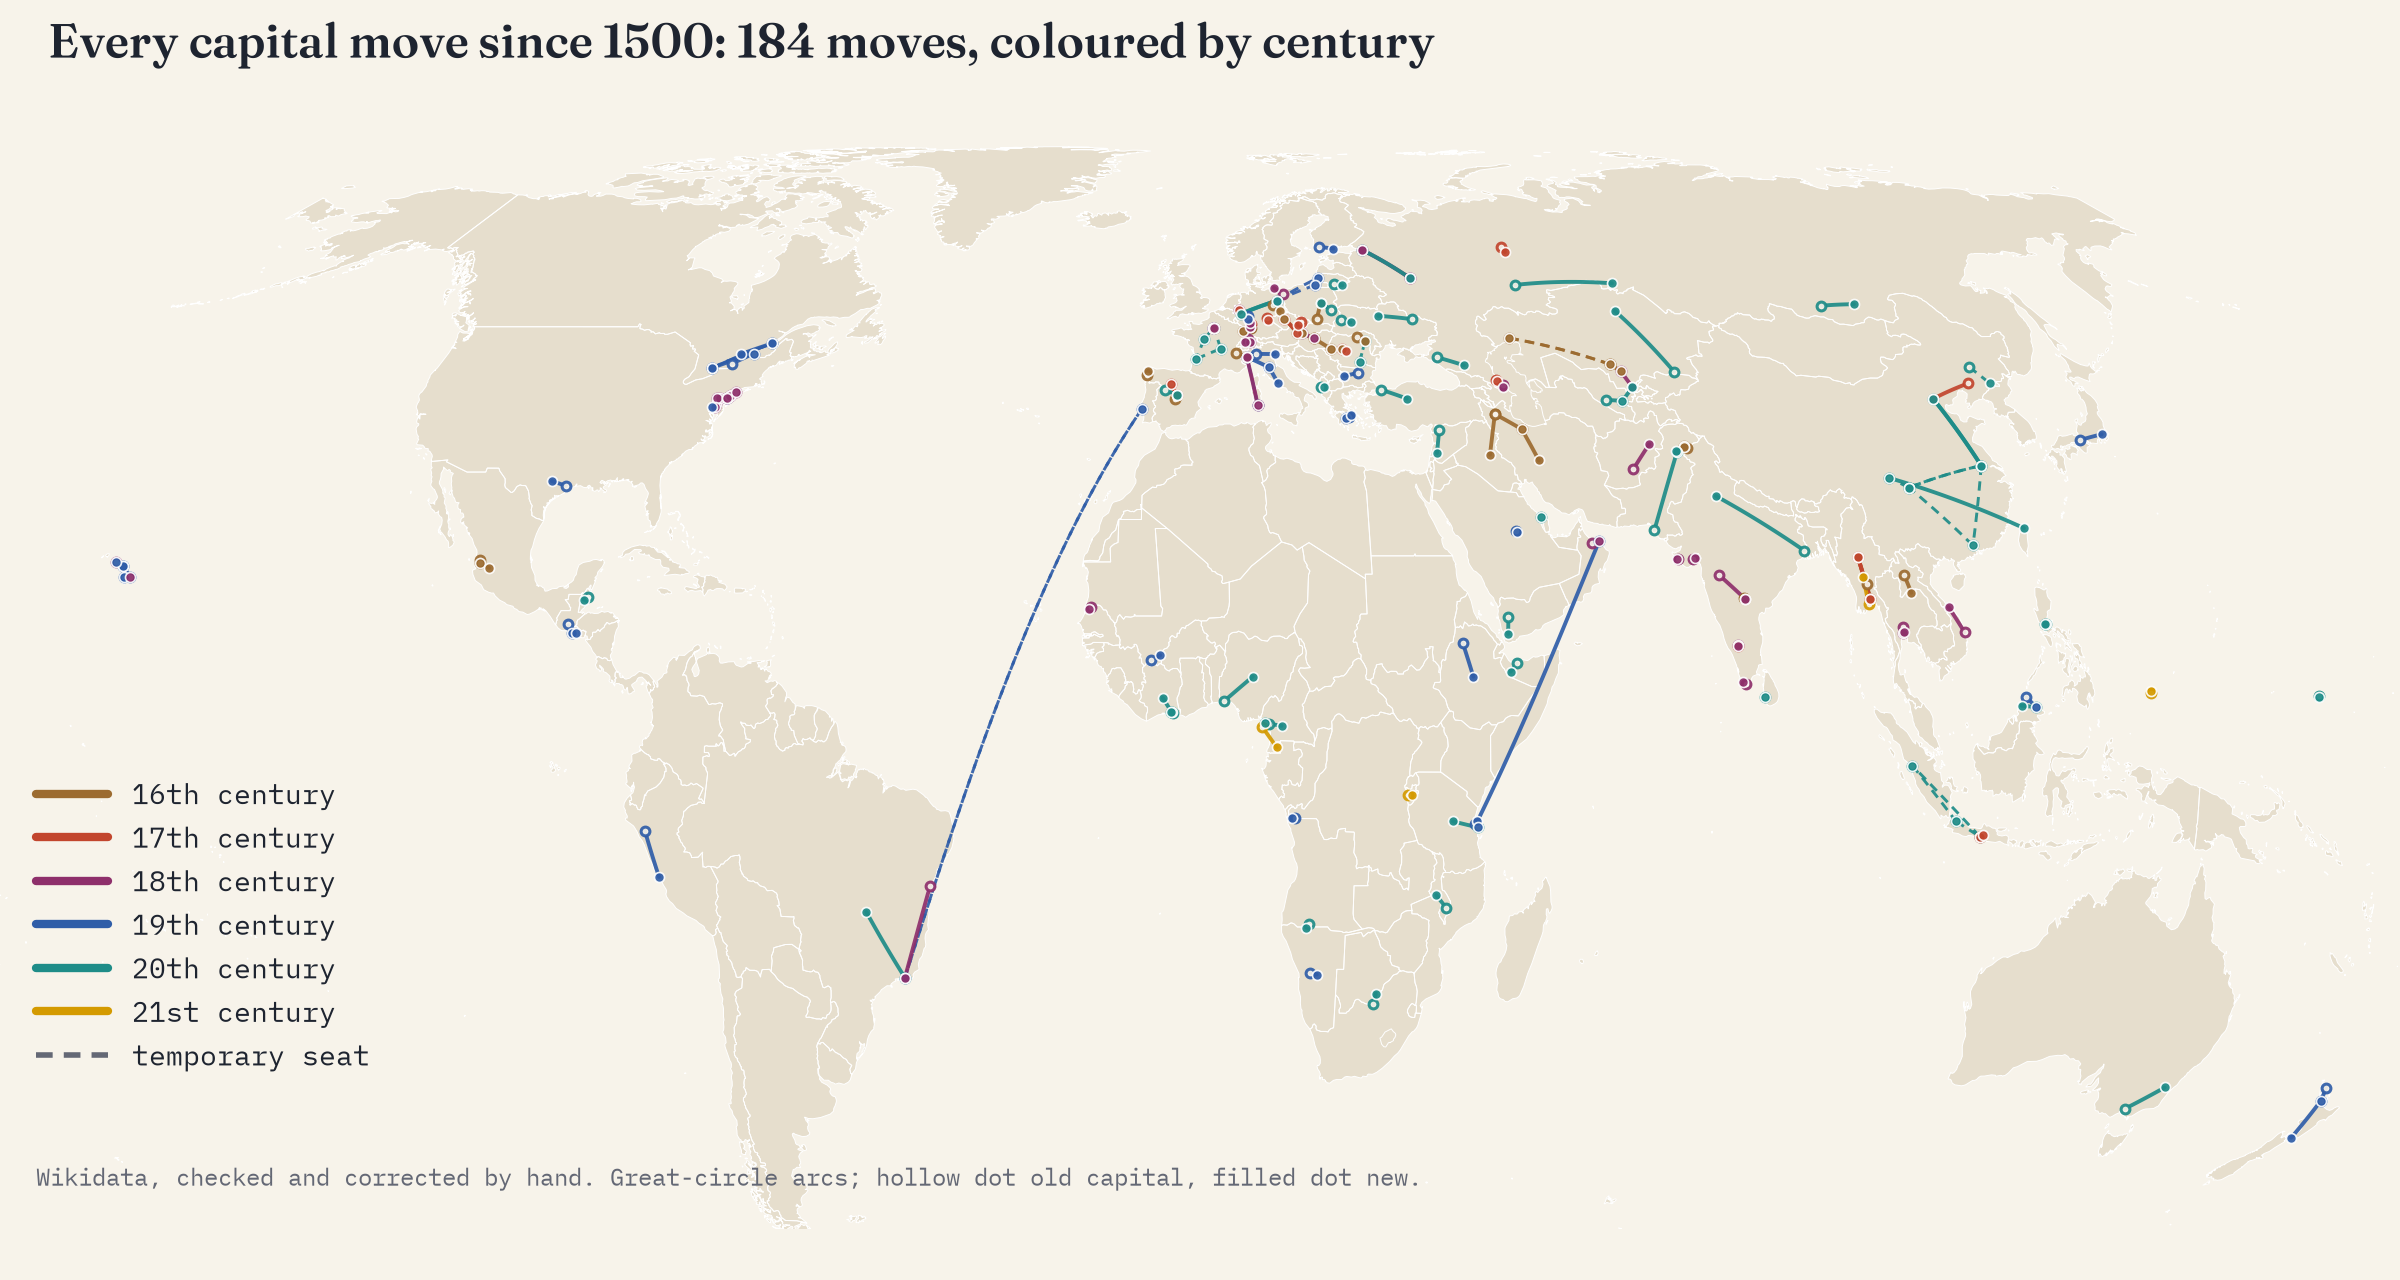
\includegraphics[width=\textwidth]{f_map.png}
\caption{Every capital move since 1500 in the table, as great-circle arcs from the old capital (hollow) to the new (filled), coloured by century; dashed arcs are temporary seats.}\label{fig:map}\end{figure}

The 20th century has the most moves, 59 (44 lasting), against 42 in the 19th and 37 in the 18th (Table~\ref{tab:century}, Figure~\ref{fig:century}). The busiest decade is the 1940s (18 moves, 7 lasting) and the busiest year 1949 (5), when the Republic of China moved from Nanjing to Guangzhou, Chongqing, Chengdu and finally Taipei. The 21st century, 26 years old, already has 4: Naypyidaw (2005), Ngerulmud (2006), Gitega (2019) and Ciudad de la Paz (2026). The low counts before 1700 partly reflect the record: Wikidata is rich for small European principalities of that period and thin for Africa, Asia and the Americas before colonial rule.

\begin{table}[tbp]\centering\small\caption{Moves by century.}\label{tab:century}\begin{tabular}{lrrrrr}\toprule Century & Moves & Lasting & Temporary & Added by hand & Median km\\\midrule
16th century & 26 & 22 & 4 & 1 & 156\\
17th century & 16 & 14 & 2 & 1 & 75\\
18th century & 37 & 24 & 13 & 9 & 133\\
19th century & 42 & 28 & 14 & 11 & 205\\
20th century & 59 & 44 & 15 & 20 & 309\\
21st century & 4 & 4 & 0 & 0 & 196\\
\midrule All & 184 & 136 & 48 & 42 & 201\\\bottomrule\end{tabular}\end{table}

\begin{figure}[tbp]\centering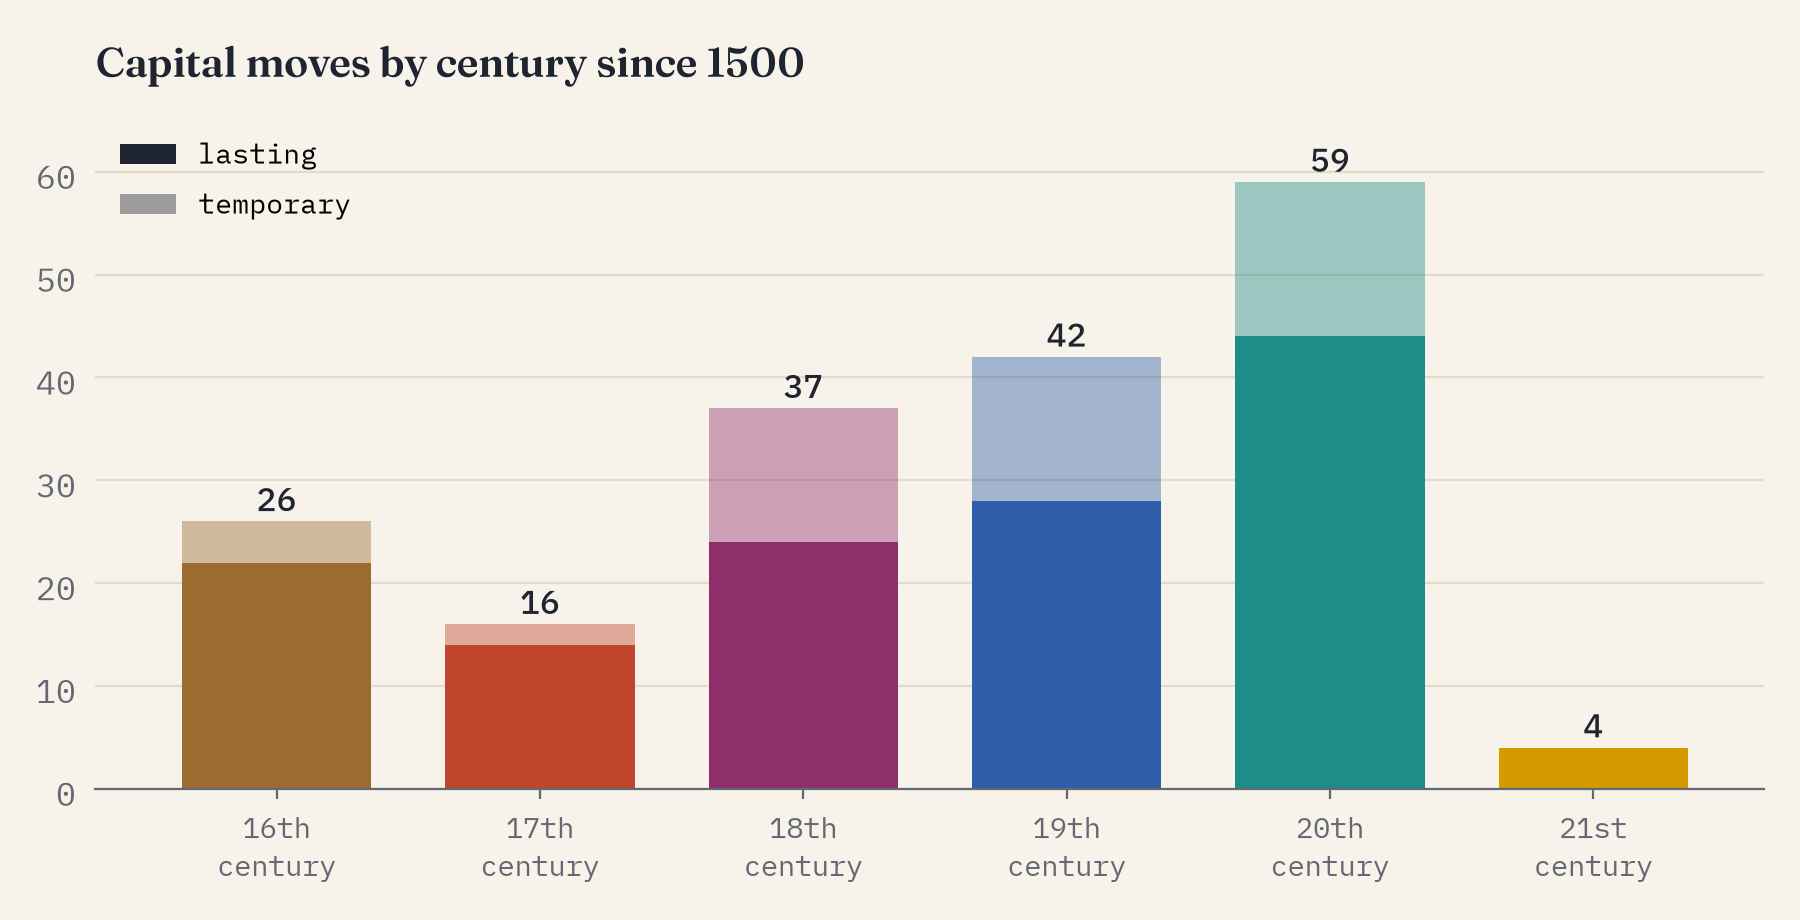
\includegraphics[width=.75\textwidth]{f_century.png}\\[0.6em]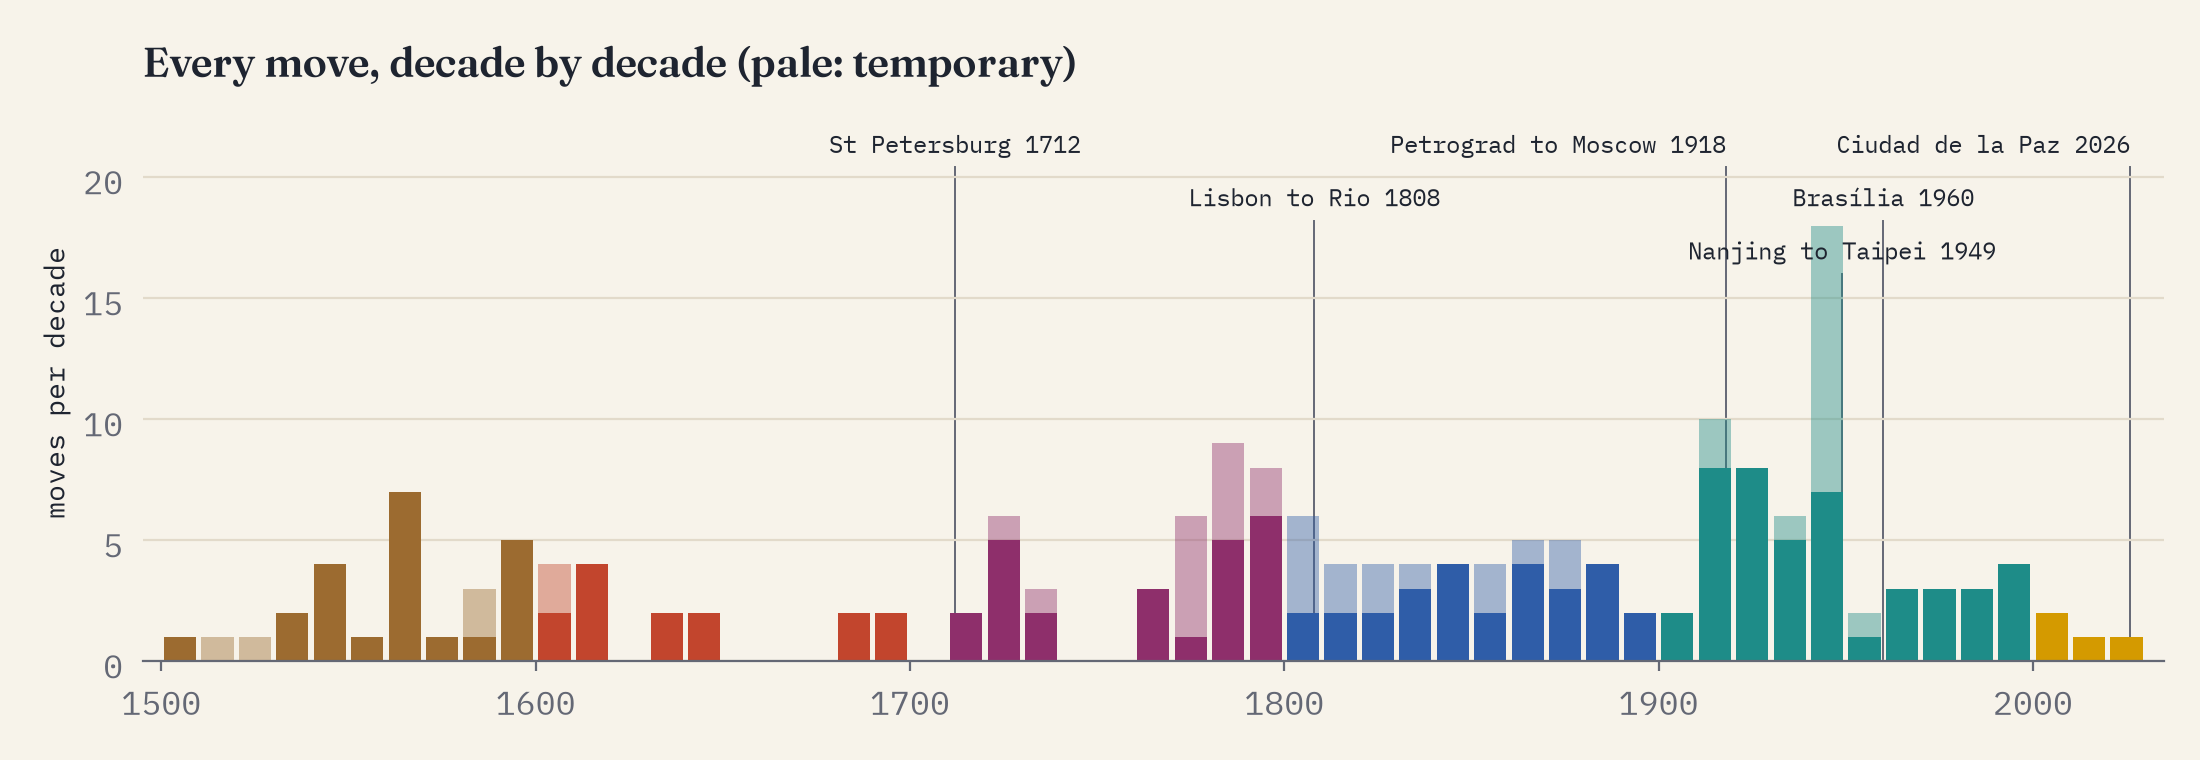
\includegraphics[width=\textwidth]{f_decade.png}
\caption{Moves by century (top) and by decade (bottom), with temporary moves pale.}\label{fig:century}\end{figure}

\subsection{How far}
Most moves are short. The median lasting move is 177 km (mean 288 km); 36\% of lasting moves are under 100 km and 21 are over 500 km. The shortest are moves across a river or to a new palace town: Thonburi to Bangkok in 1782 (4 km), Muharraq to Manama in 1921, Durlach to Karlsruhe in 1715. The longest is the Portuguese court's flight from Napoleon, Lisbon to Rio de Janeiro in 1808 (7,716 km), twice the next (Table~\ref{tab:longest}, Figure~\ref{fig:longest}). The longest lasting move is Said bin Sultan's transfer of the Omani capital from Muscat to Stone Town, Zanzibar, in 1840 (3,924 km), followed by Chengdu to Taipei (1,828 km) and Calcutta to Delhi (1,305 km). 14 moves exceed 1{,}000 km.

\begin{table}[tbp]\centering\small\caption{The ten longest moves since 1500 (great-circle distance).}\label{tab:longest}\begin{tabular}{llp{4.6cm}rl}\toprule Move & Year & State & km & Kind\\\midrule
Lisbon to Rio de Janeiro & 1808 & Kingdom of Portugal & 7,716 & temporary\\
Muscat to Zanzibar & 1840 & Omani Empire & 3,924 & lasting\\
Chengdu to Taipei & 1949 & Republic of China & 1,828 & lasting\\
Yogyakarta to Bukittinggi & 1948 & Indonesia & 1,388 & temporary\\
Calcutta to Delhi & 1911 & British Raj & 1,305 & lasting\\
Sighnaq to Saray-Jük & 1511 & Kazakh Khanate & 1,235 & temporary\\
Saray-Jük to Sighnaq & 1521 & Kazakh Khanate & 1,235 & temporary\\
Salvador to Rio de Janeiro & 1763 & State of Brazil & 1,211 & lasting\\
Nanjing to Chongqing & 1937 & Republic of China & 1,200 & temporary\\
Chongqing to Nanjing & 1946 & Republic of China & 1,200 & temporary\\
\bottomrule\end{tabular}\end{table}

\begin{figure}[tbp]\centering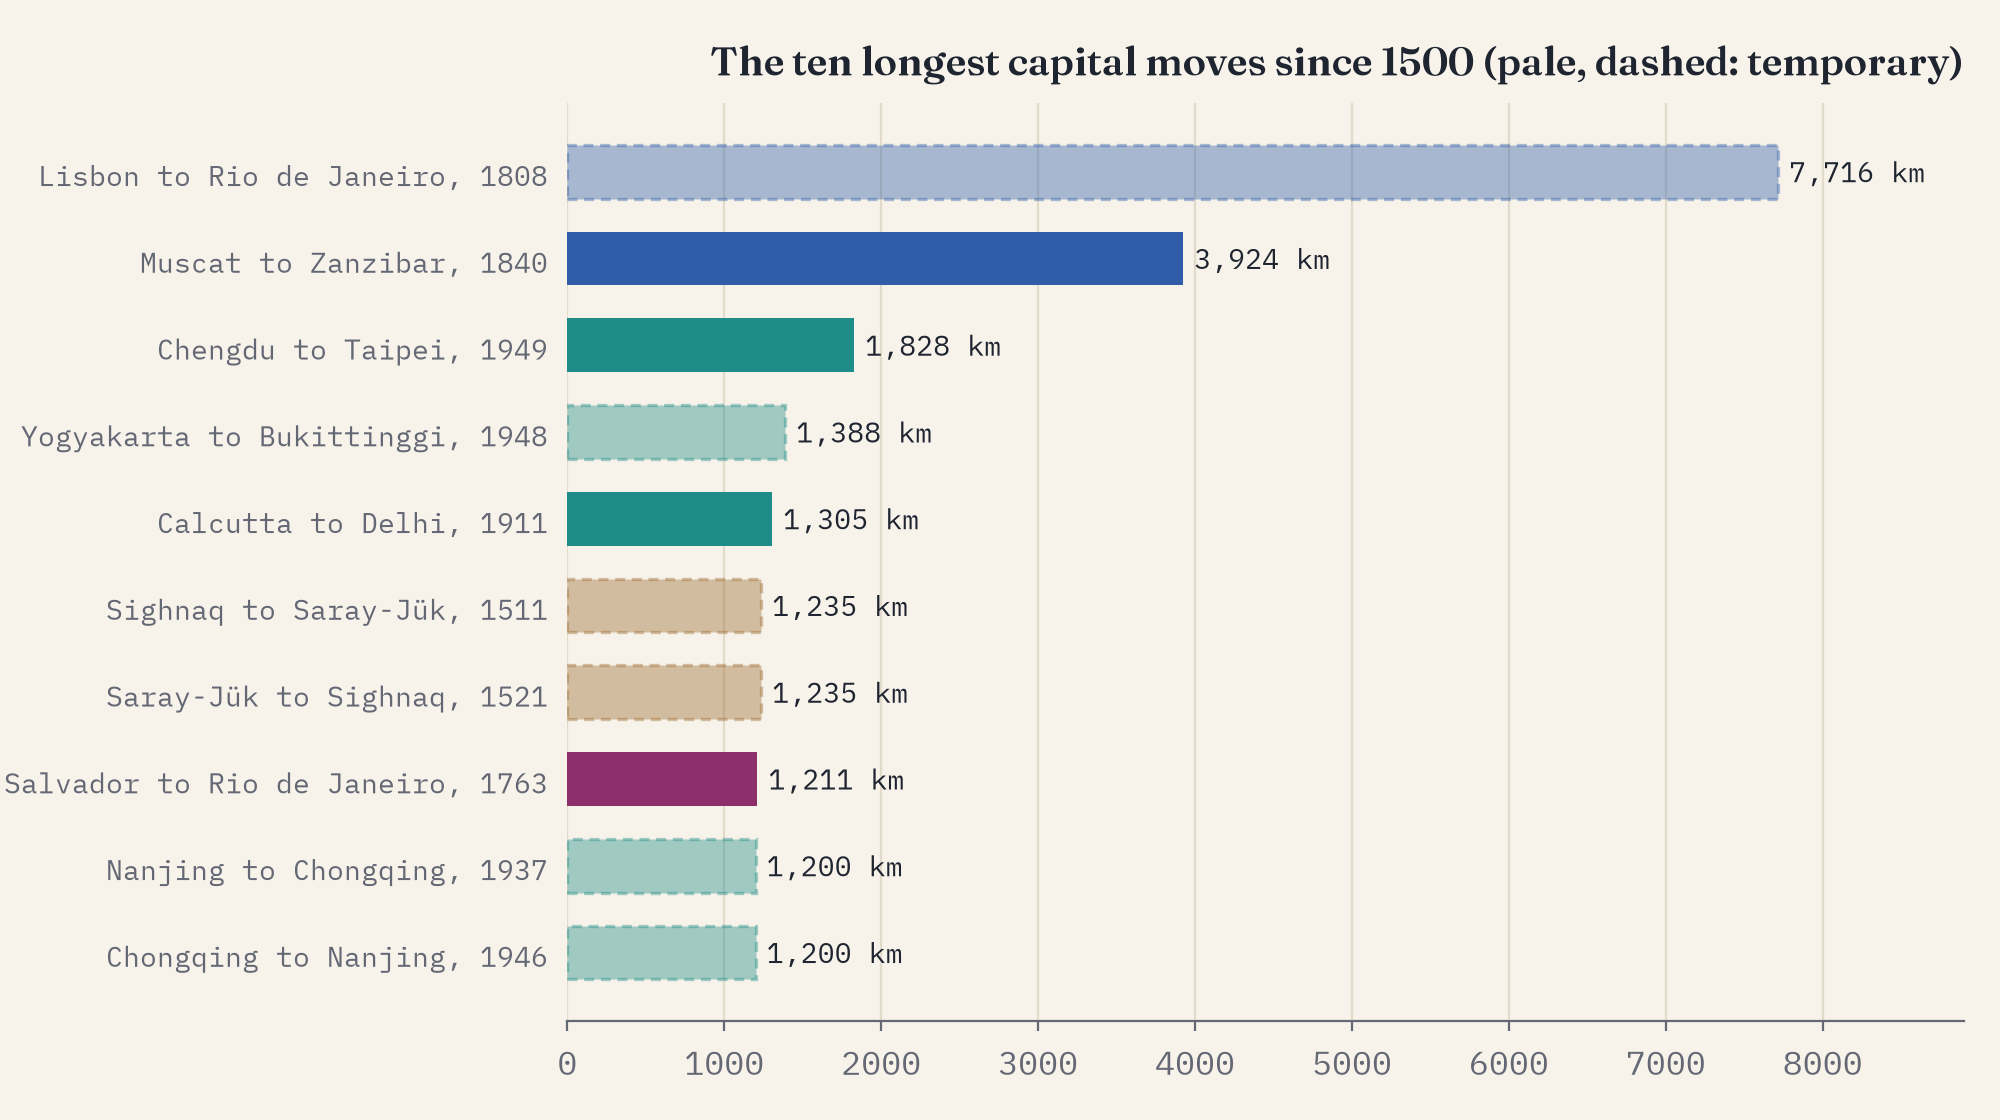
\includegraphics[width=.86\textwidth]{f_longest.png}
\caption{The ten longest moves; pale, dashed bars are temporary seats.}\label{fig:longest}\end{figure}

\subsection{Capitals built for the purpose}
17 moves went to a city founded, or laid out as a new town, to be a capital (Figure~\ref{fig:purpose}). Early examples are palace and residence towns (Versailles, Karlsruhe) and St Petersburg; Washington was planned from 1791. 12 of the 17 came after 1900: New Delhi, Canberra, Quezon City, Brasília, Gaborone, Islamabad, Belmopan, Palikir, Abuja, Naypyidaw, Ngerulmud and Ciudad de la Paz. They are 25\% of all lasting moves since 1900. Several famous relocations went to existing towns rather than new ones (Ankara, Dodoma, Yamoussoukro, Lilongwe, Astana, formerly Akmola) and are not counted as purpose-built.

\begin{figure}[tbp]\centering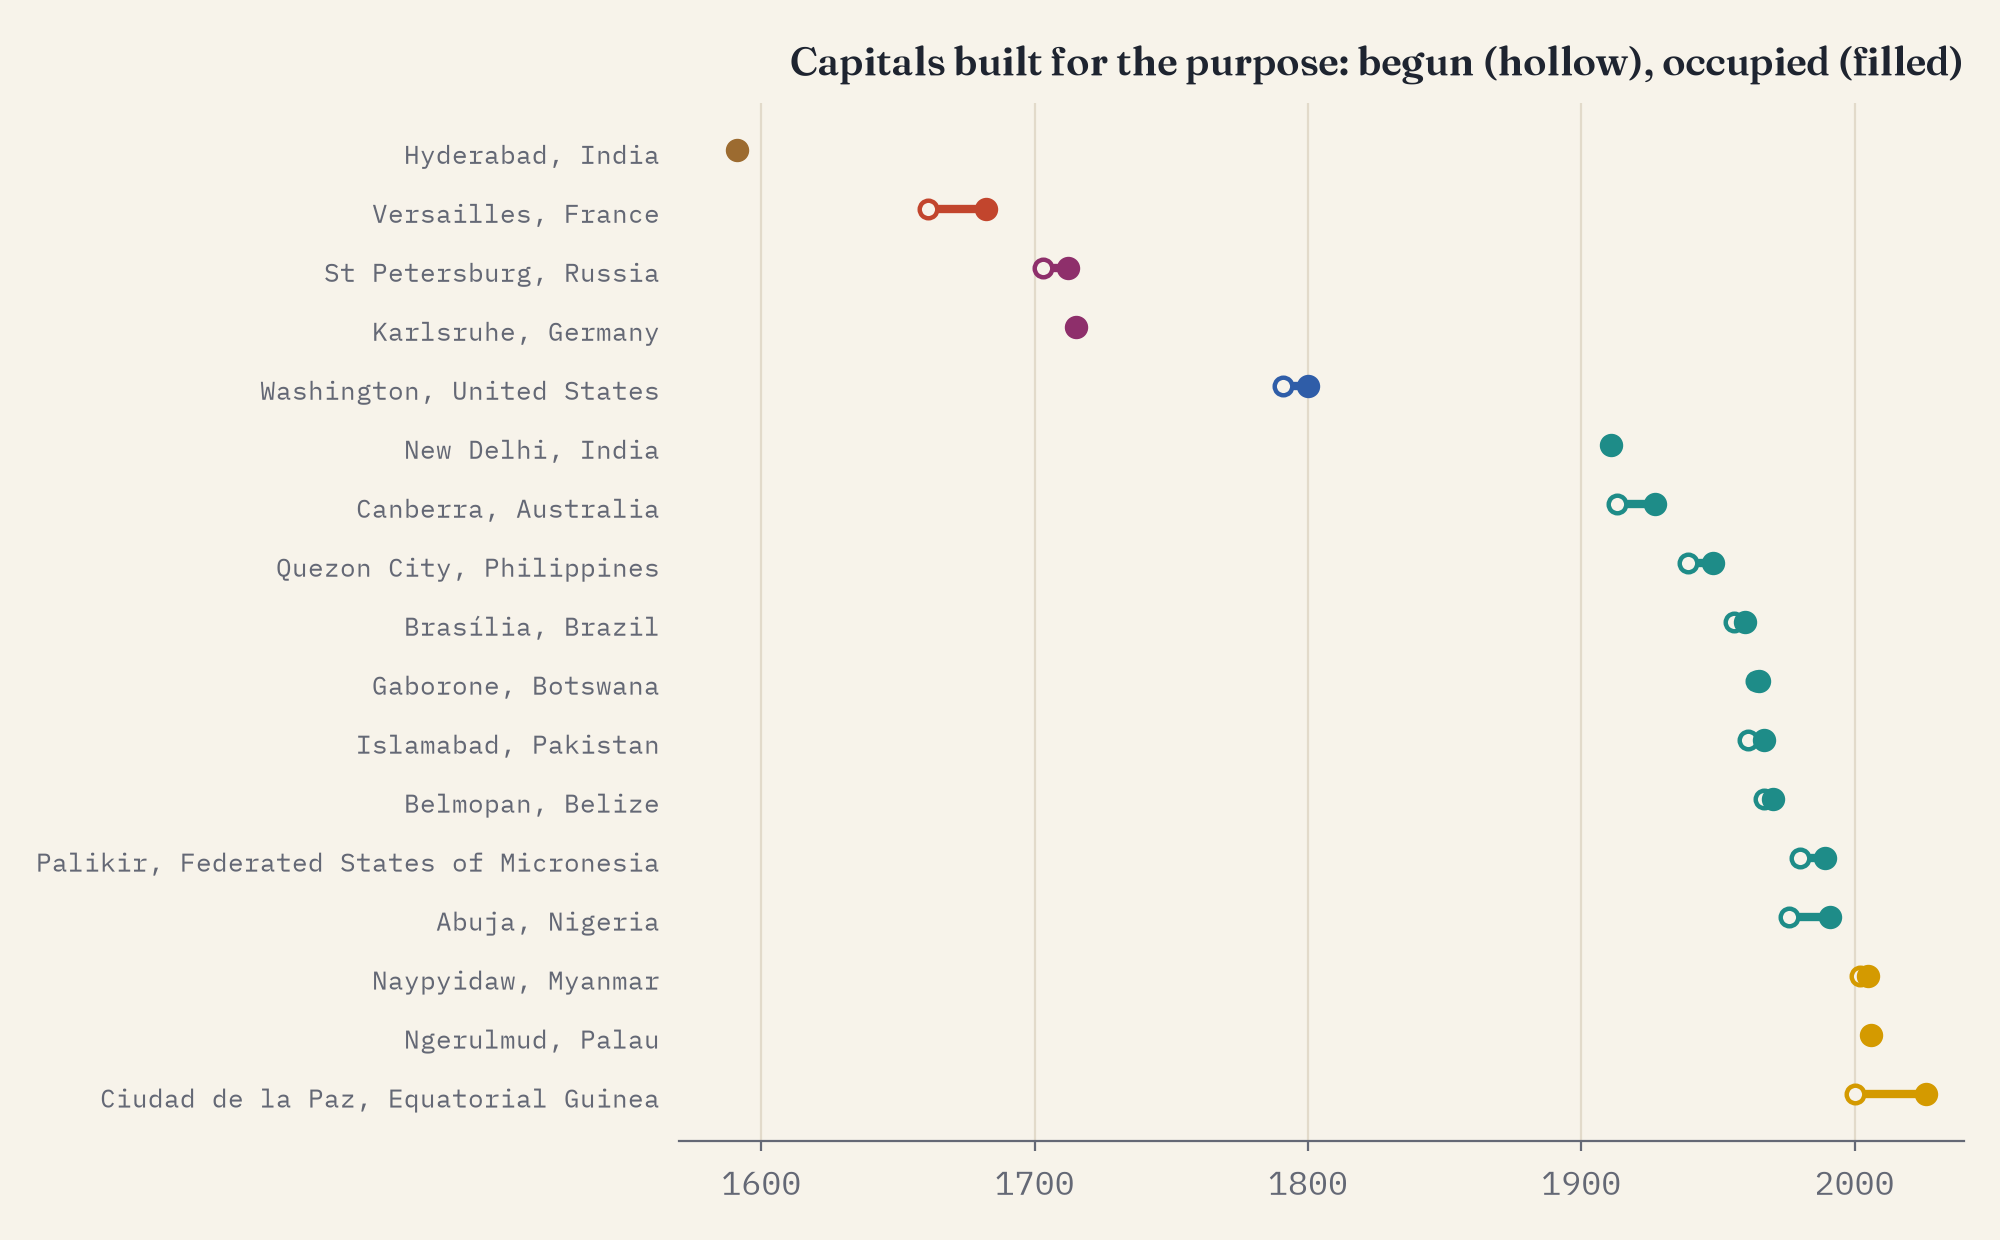
\includegraphics[width=.86\textwidth]{f_purpose.png}
\caption{Purpose-built capitals: when building began or the city was founded (hollow) and when the government moved in (filled).}\label{fig:purpose}\end{figure}

\subsection{Inland and towards the centre}
Of 48 lasting moves since 1900, 13 (27\%) left a capital within 50 km of the sea for one at least 50 km further inland, against 7 of 88 (8\%) before 1900 (Figure~\ref{fig:sea}). The pattern is the post-colonial and nation-building move from a port to the interior: Rio to Brasília, Lagos to Abuja, Dar es Salaam to Dodoma, Abidjan to Yamoussoukro, Yangon to Naypyidaw, Karachi to Rawalpindi and Islamabad, Malabo to Ciudad de la Paz; Melbourne to Canberra and Istanbul to Ankara fit it too. Only 1 went the other way, the Republic of China's retreat to Taipei. Of 45 lasting moves since 1900 within one present-day country, 25 brought the capital at least 25 km closer to the centroid of the country's main landmass and 11 took it further away; Brasília is 916 km closer to Brazil's centre than Rio, Abuja 535 km closer to Nigeria's than Lagos. Directions are otherwise mixed: 24 lasting moves went east and 11 north.

\begin{figure}[tbp]\centering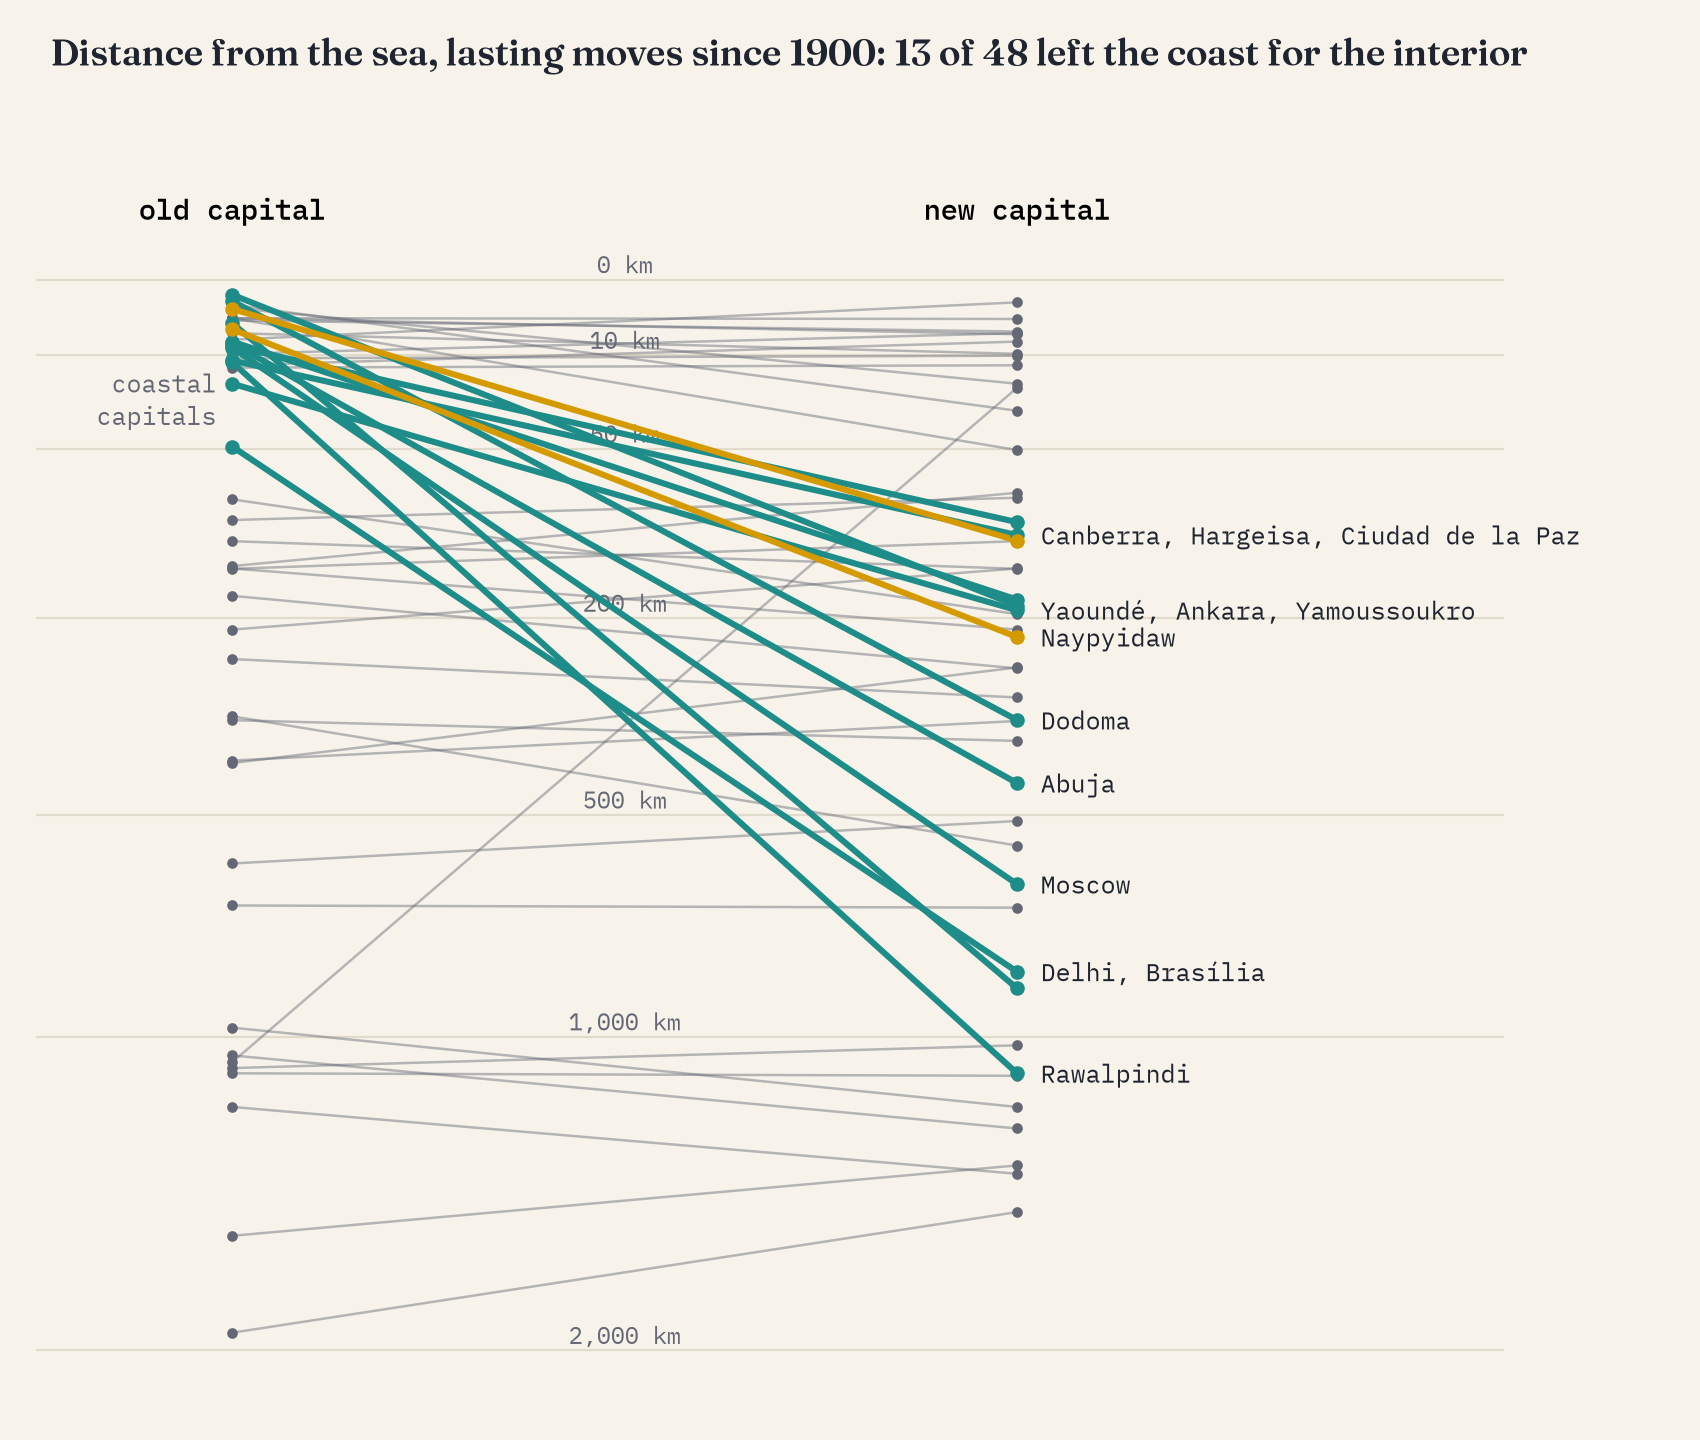
\includegraphics[width=.72\textwidth]{f_sea.png}
\caption{Distance from the sea of the old and new capital, lasting moves since 1900 (square-root scale). Coloured: from the coast to the interior.}\label{fig:sea}\end{figure}

\subsection{Who moved most}
By present-day country the United States has the most moves (17, 5 lasting), 11 of them the Continental Congress and early federal government between 1776 and 1800, the rest the Kingdom of Hawai'i and the Republic of Texas (Figure~\ref{fig:countries}). Germany follows with 12, from 8 separate states, then India and China (10 each) and Russia and France (9 each). Counted by state, the most mobile are the United States (11), the Republic of China (8), France (7) and the Province of Canada (6), whose parliament alternated between Toronto and Quebec City before settling in Ottawa. 35 present-day countries have two or more moves. These counts measure the record as much as restlessness: they are highest where Wikidata or my additions are most detailed.

\begin{figure}[tbp]\centering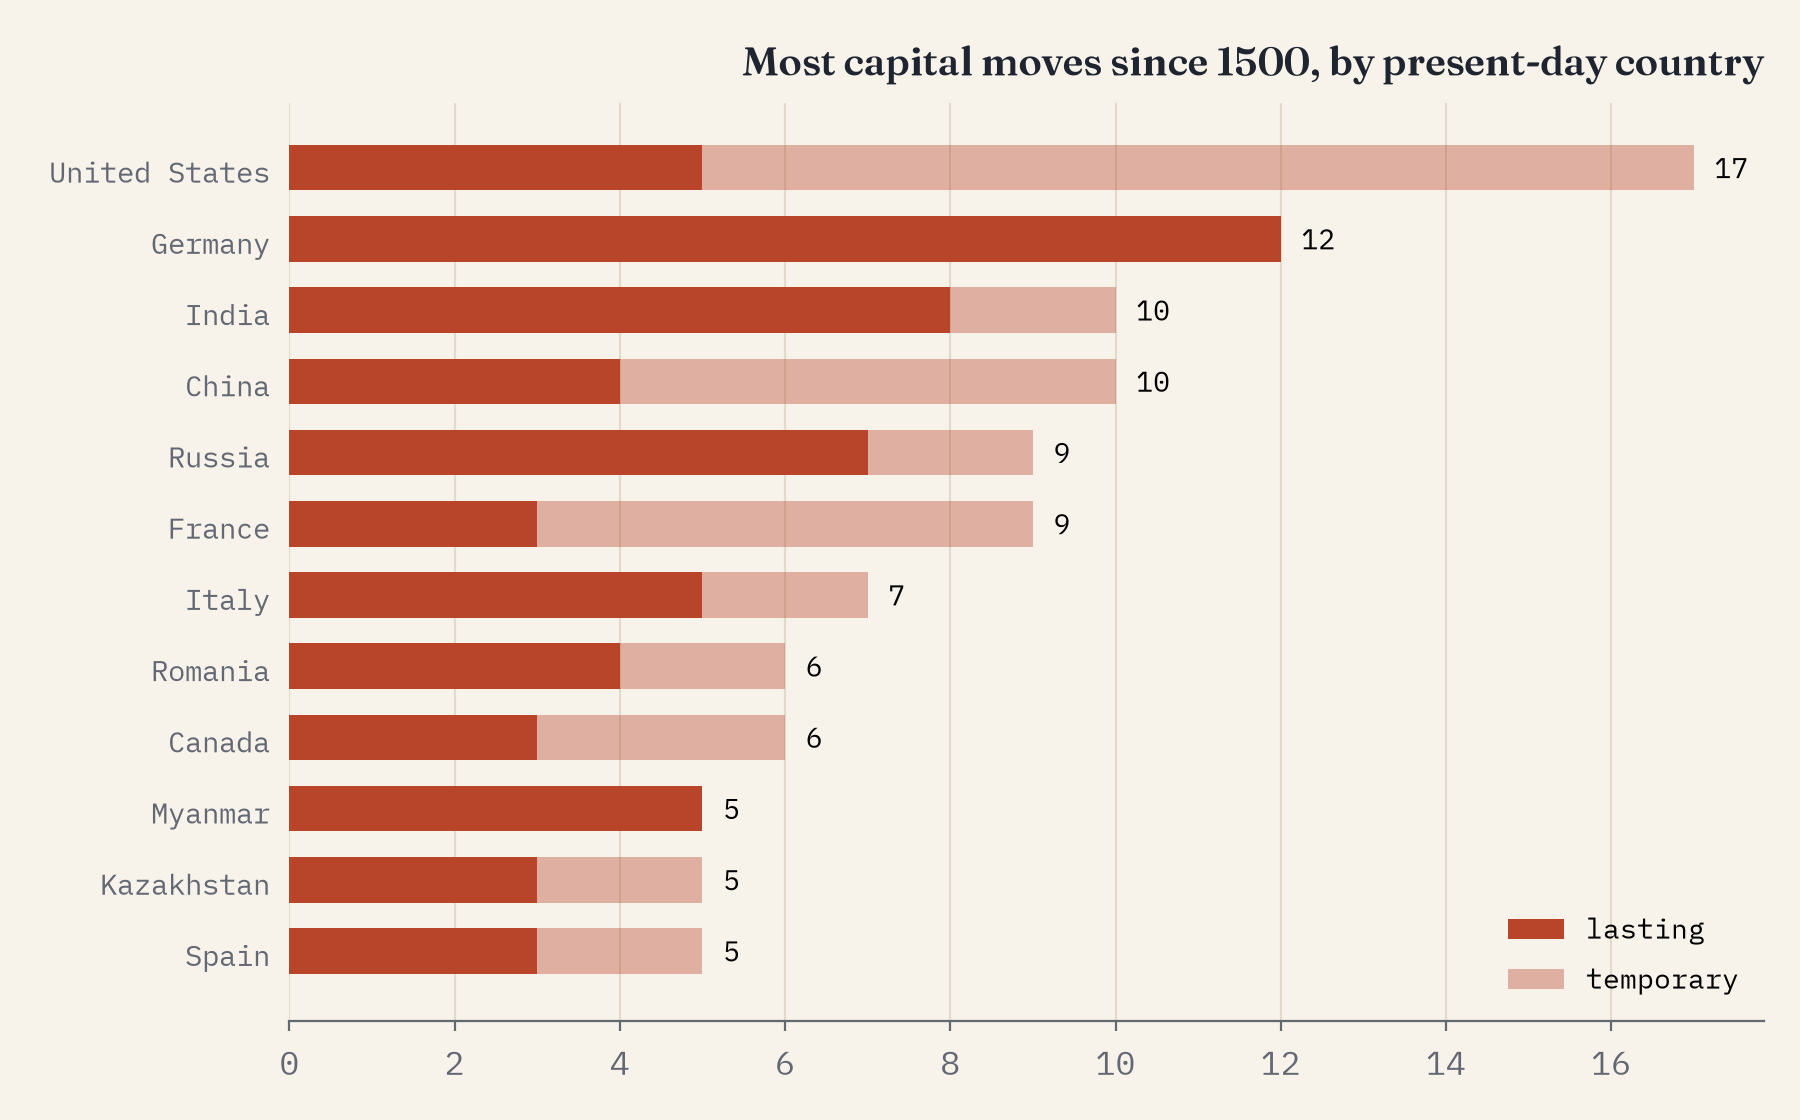
\includegraphics[width=.8\textwidth]{f_countries.png}
\caption{Most moves since 1500 by present-day country; pale: temporary.}\label{fig:countries}\end{figure}

\begin{figure}[tbp]\centering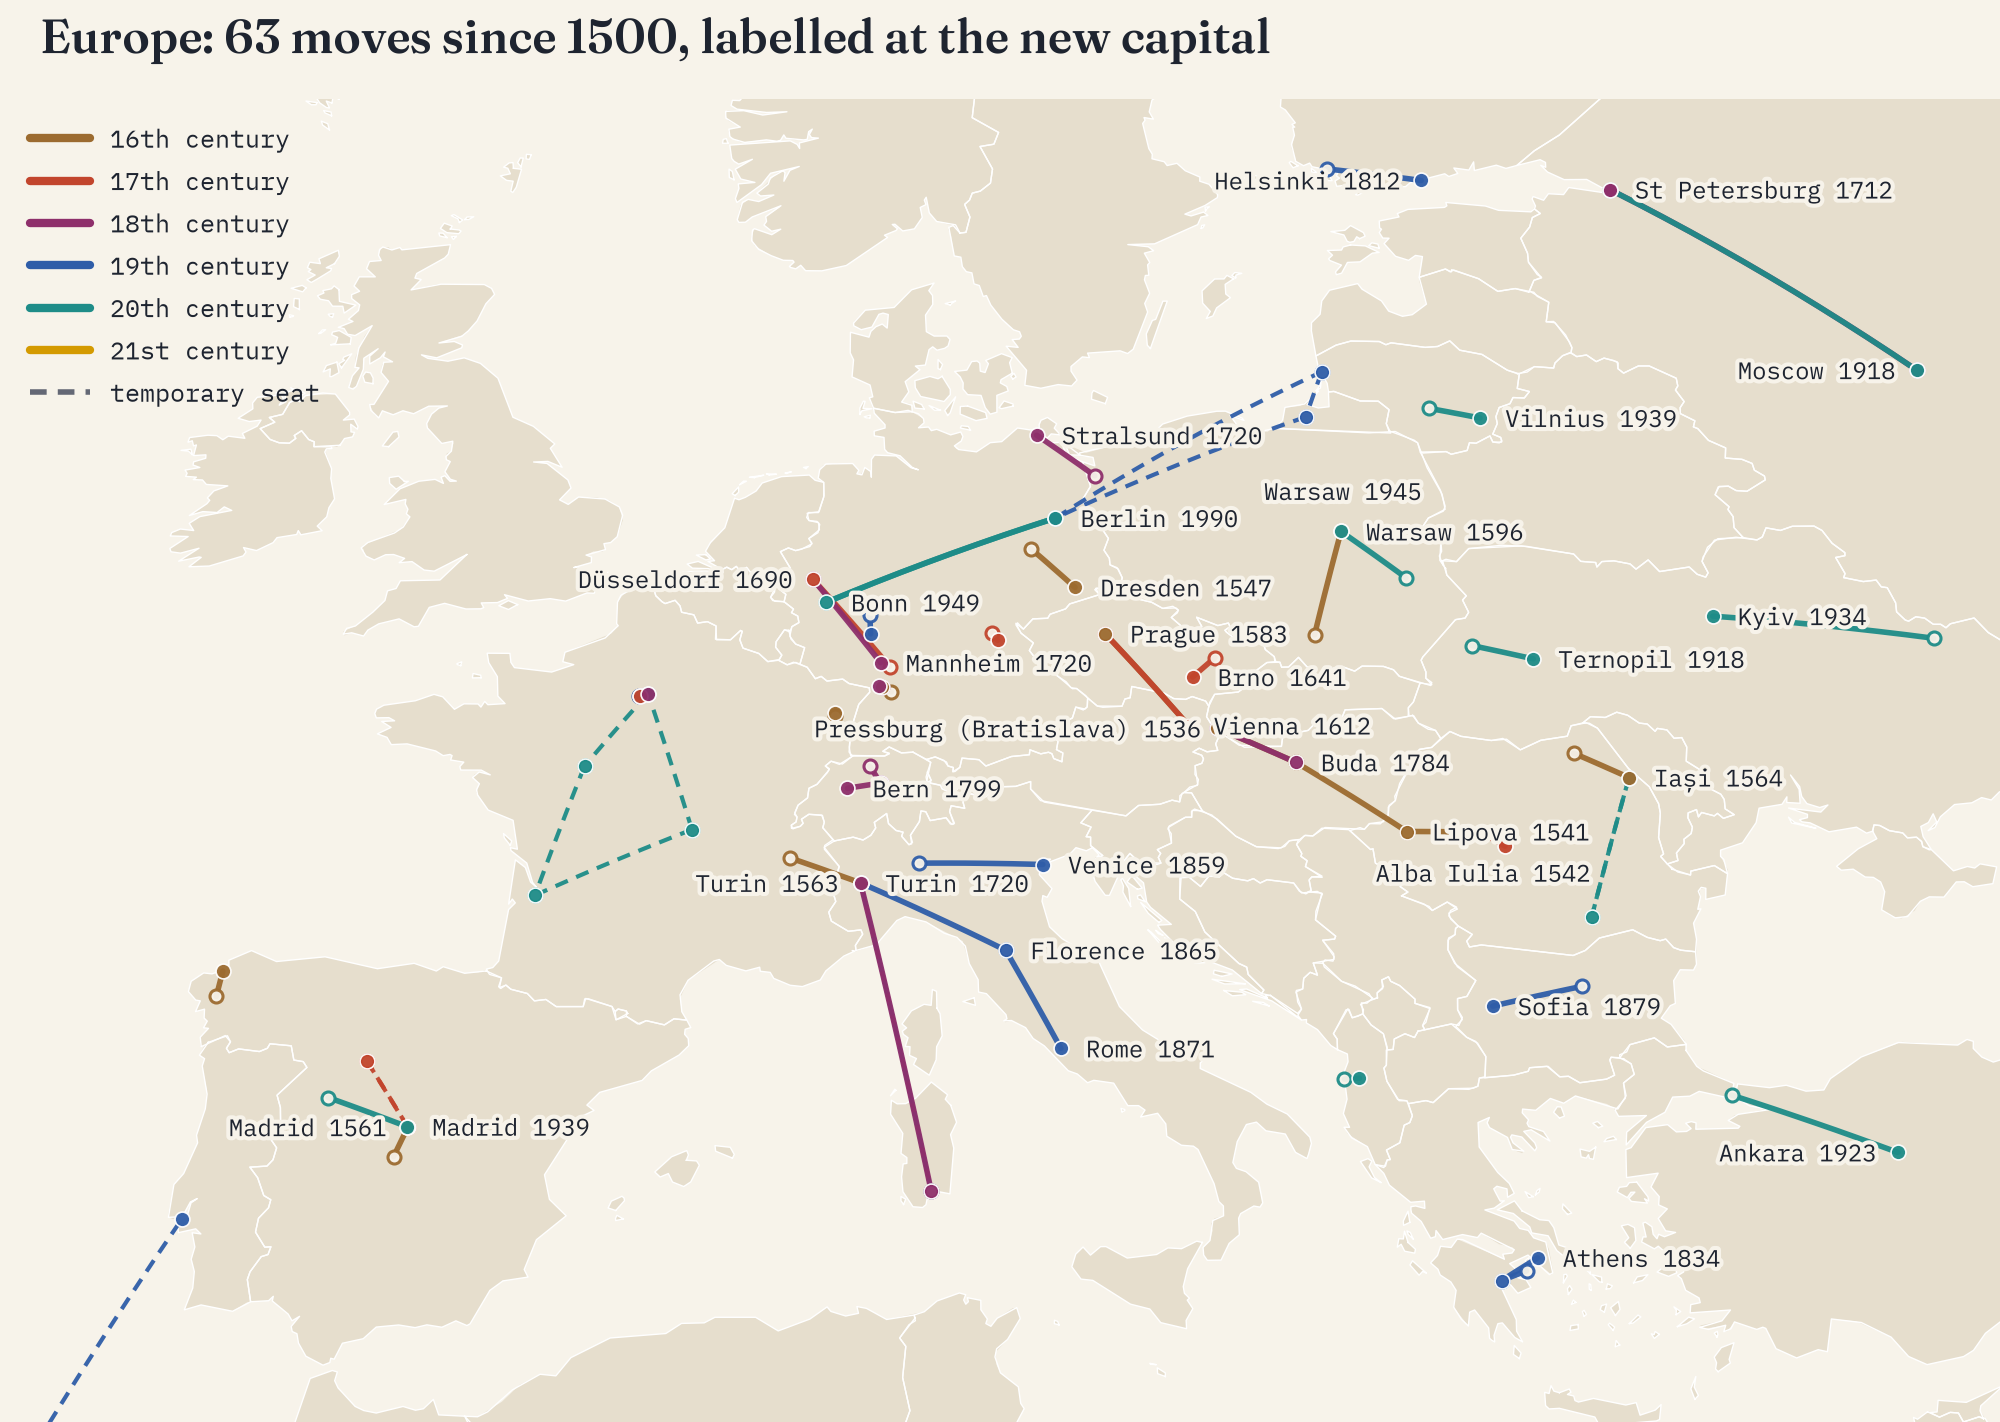
\includegraphics[width=.86\textwidth]{f_europe.png}
\caption{Europe, where the record is densest, labelled at the new capital.}\label{fig:europe}\end{figure}

\subsection{The famous moves}
Of the 24 famous moves in Table~\ref{tab:famous}, 18 were in Wikidata, several recorded twice or with a second, wrong year; the rest had to be added. Tanzania's and Côte d'Ivoire's moves are dated by the decision or the move of the legislature, not of the whole government: Dodoma was chosen in 1973, the National Assembly moved in 1996 and most ministries around 2019, and most of the government stayed in Abidjan after 1983. Germany's capital became Berlin on reunification in 1990, but the government moved from Bonn only in 1999.

\begin{table}[tbp]\centering\scriptsize\caption{The famous moves checked by hand: whether Wikidata had them, and the source used.}\label{tab:famous}\begin{tabular}{>{\raggedright\arraybackslash}p{3.6cm}l>{\raggedright\arraybackslash}p{3.2cm}r>{\raggedright\arraybackslash}p{2.2cm}>{\raggedright\arraybackslash}p{3.6cm}}\toprule Move & Year & State & km & Status & Source\\\midrule
Rio de Janeiro to Brasília & 1960 & Brazil & 931 & in Wikidata, checked & WP: Brasília\\
Calcutta to Delhi & 1911 & British Raj & 1,305 & in Wikidata, checked & WP: New Delhi\\
St Petersburg to Moscow & 1728 & Russian Empire & 635 & in Wikidata, checked & \\
St Petersburg to Moscow & 1918 & Russian Socialist Federative Soviet Republic & 635 & in Wikidata, checked & WP: Moscow\\
Istanbul to Ankara & 1923 & Republic of Turkey & 349 & added by hand & WP: Ankara\\
Lagos to Abuja & 1991 & Nigeria & 536 & in Wikidata, checked & WP: Abuja\\
Karachi to Rawalpindi & 1959 & Pakistan & 1,135 & added by hand & WP: Islamabad\\
Rawalpindi to Islamabad & 1967 & Pakistan & 11 & in Wikidata, checked & WP: Islamabad\\
Almaty to Astana & 1997 & Kazakhstan & 970 & in Wikidata, checked & WP: Astana\\
Yangon to Naypyidaw & 2005 & Myanmar & 328 & in Wikidata, checked & WP: Naypyidaw\\
Dar es Salaam to Dodoma & 1996 & Tanzania & 397 & in Wikidata, checked & WP: Dodoma\\
Abidjan to Yamoussoukro & 1983 & Ivory Coast & 215 & in Wikidata, checked & WP: Yamoussoukro\\
Berlin to Bonn & 1949 & Germany & 476 & in Wikidata, checked & WP: Bonn\\
Bonn to Berlin & 1990 & Germany & 476 & in Wikidata, checked & WP: Berlin/Bonn Act\\
Melbourne to Canberra & 1927 & Australia & 466 & in Wikidata, checked & WP: Canberra\\
Kyoto to Tokyo & 1868 & Japan & 364 & added by hand & WP: Tokyo\\
Lisbon to Rio de Janeiro & 1808 & Kingdom of Portugal & 7,716 & in Wikidata, checked & WP: Transfer of the Portuguese cou\\
Rio de Janeiro to Lisbon & 1821 & Portuguese Empire & 7,716 & in Wikidata, checked & WP: Transfer of the Portuguese cou\\
New York to Philadelphia & 1790 & United States & 130 & in Wikidata, checked & WP: List of capitals in the United\\
Philadelphia to Washington & 1800 & United States & 199 & in Wikidata, checked & WP: List of capitals in the United\\
Quebec City to Ottawa & 1866 & Province of Canada & 379 & added by hand & WP: Canadian seat of government di\\
Beijing to Nanjing & 1928 & Republic of China & 898 & added by hand & WP: Capital of the Republic of Chi\\
Nanjing to Beijing & 1912 & Republic of China & 898 & added by hand & WP: Capital of the Republic of Chi\\
Mukden (Shenyang) to Beijing & 1644 & Qing dynasty & 627 & in Wikidata, checked & WP: Shenyang\\
\bottomrule\end{tabular}\end{table}

\subsection{Moves planned, and one made in 2026}
Indonesia's planned move to Nusantara, in East Kalimantan (1,240 km from Jakarta), has not been made. A 2022 law names Nusantara as the new capital, but the transfer takes effect only with a presidential decree, which had not been issued; in May 2026 the Constitutional Court confirmed that Jakarta remains the capital until it is \citep{star,jakpost}, and the government's stated aim is to make Nusantara a ``political capital'' by 2028. Wikidata marks Nusantara's capital statement as deprecated. Equatorial Guinea's move to Ciudad de la Paz, by a decree reported in January 2026 that gave government bodies a year to relocate \citep{africanews}, is included as the newest move.

\section{Limitations}
The table is a reading of an open, collaboratively edited database, corrected where I checked it, not a complete history. It misses moves that Wikidata does not record and I did not add, and its coverage is far richer for Europe, and for colonial administrations, than for pre-colonial Africa, Asia and the Americas. ``Capital'' means the state's recorded capital, which for early modern monarchies is often the court or a ruler's residence; several countries divide the functions of a capital (Bolivia, the Netherlands, South Africa, Benin, Malaysia), and some moves transferred the title or parliament long before the ministries. Dates in Wikidata for medieval and early modern states are often rounded to the year and sometimes disputed, so ``high'' confidence means internal consistency, not historical certainty. Most hand checks rest on English Wikipedia articles, which are themselves secondary. The classification of temporary moves and of purpose-built capitals involves judgement, set out in the code. Distances are between the coordinates Wikidata gives for each city, so short moves within a growing city (Rawalpindi to Islamabad, 11 km) depend on where those points lie.

\section{Conclusion}
Capital moves are common: 184 since 1500 in this table, with the 20th century the busiest and the planned interior capital its signature. The open record can produce such a table, but not on its own. Its dates are sparse, its items overlap, and several of the best-known moves are missing or misplaced, so a reusable table needs explicit rules, hand checking and a full log of the edits. That log is part of the contribution: it shows where Wikidata could be improved, and the data, code and edits are released so that others can extend them.

\section*{Data and code availability}
Data (moves, manual edits with sources, renamings set aside, planned moves, results) and code are at \url{https://github.com/Tristan-Hotham/moving-capitals} and archived with this paper at \href{https://doi.org/10.5281/zenodo.23847842}{https://doi.org/10.5281/zenodo.23847842}. Interactive version: \url{https://maps.tristanhotham.com/moving-capitals/}. Wikidata is CC0; Natural Earth is public domain. This paper, the figures and the derived data are released under CC BY 4.0; code under MIT.

\section*{AI statement}
I wrote the text, with drafting and editing assistance from Claude (Anthropic), which also helped prepare the analysis code. I reviewed and checked all text and results.

\begin{thebibliography}{9}
\bibitem[africanews(2026)]{africanews} africanews (2026) Equatorial Guinea relocates capital. \url{https://www.africanews.com/2026/01/05/equatorial-guinea-relocates-capital/}
\bibitem[Gordon(2006)]{gordon} Gordon, D. L. A. (ed.) (2006) \emph{Planning Twentieth Century Capital Cities}. London: Routledge.
\bibitem[Natural Earth(2026)]{naturalearth} Natural Earth (2026) Admin 0 countries, land and populated places, 1:50m and 1:10m. Public domain. \url{https://www.naturalearthdata.com/}
\bibitem[QLever(2026)]{qlever} Bast, H. and Buchhold, B. QLever SPARQL engine, Wikidata endpoint. \url{https://qlever.cs.uni-freiburg.de/wikidata}
\bibitem[Rossman(2017)]{rossman} Rossman, V. (2017) \emph{Capital Cities: Varieties and Patterns of Development and Relocation}. London: Routledge.
\bibitem[Schatz(2004)]{schatz} Schatz, E. (2004) What capital cities say about state and nation building. \emph{Nationalism and Ethnic Politics}, 9(4), 111 to 140.
\bibitem[The Jakarta Post(2026)]{jakpost} The Jakarta Post (2026) Court ruling raises further questions over Nusantara's future. \url{https://www.thejakartapost.com/indonesia/2026/05/15/court-ruling-raises-further-questions-over-nusantaras-future.html}
\bibitem[The Star(2026)]{star} The Star (2026) Court ruling raises further questions over future of Indonesia's Nusantara. \url{https://www.thestar.com.my/aseanplus/aseanplus-news/2026/05/15/court-ruling-raises-further-questions-over-future-of-indonesia039s-nusantara}
\bibitem[Vrande\v{c}i\'c and Kr\"otzsch(2014)]{wikidata} Vrande\v{c}i\'c, D. and Kr\"otzsch, M. (2014) Wikidata: a free collaborative knowledgebase. \emph{Communications of the ACM}, 57(10), 78 to 85.
\bibitem[Wikipedia(2026)]{wikiplanned} Wikipedia contributors (2026) Planned capital. \emph{English Wikipedia}. \url{https://en.wikipedia.org/wiki/Planned_capital}
\end{thebibliography}
\end{document}
